\section{Evaluation}
\label{sec:evaluation}

Let us now see how well on-demand evaluation works in practice.
We begin by empirically studying the bias and variance of the joint estimator proposed in \refsec{method} and find it is able to correct for pooling bias while significantly reducing variance in comparison with the simple estimator.
We then ask if on-demand evaluation can serve as a practical replacement for the TAC KBP evaluations by comparing the scores predicted by our framework with the official evaluation on TAC KBP 2016 document corpus.
We find that we are able to obtain results of comparable quality in a cost effective manner.

\begin{figure*}[t]
  \centering
  \begin{subfigure}{0.49\textwidth}
    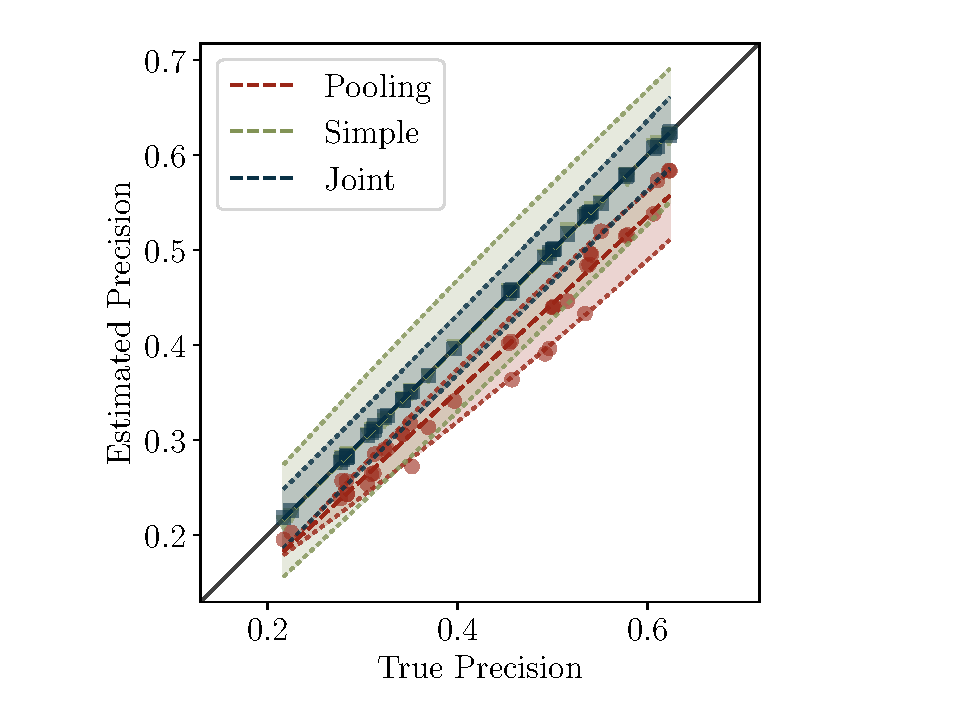
\includegraphics[width=\textwidth]{figures/simulation/simulation-p}
  \end{subfigure}
  \begin{subfigure}{0.49\textwidth}
    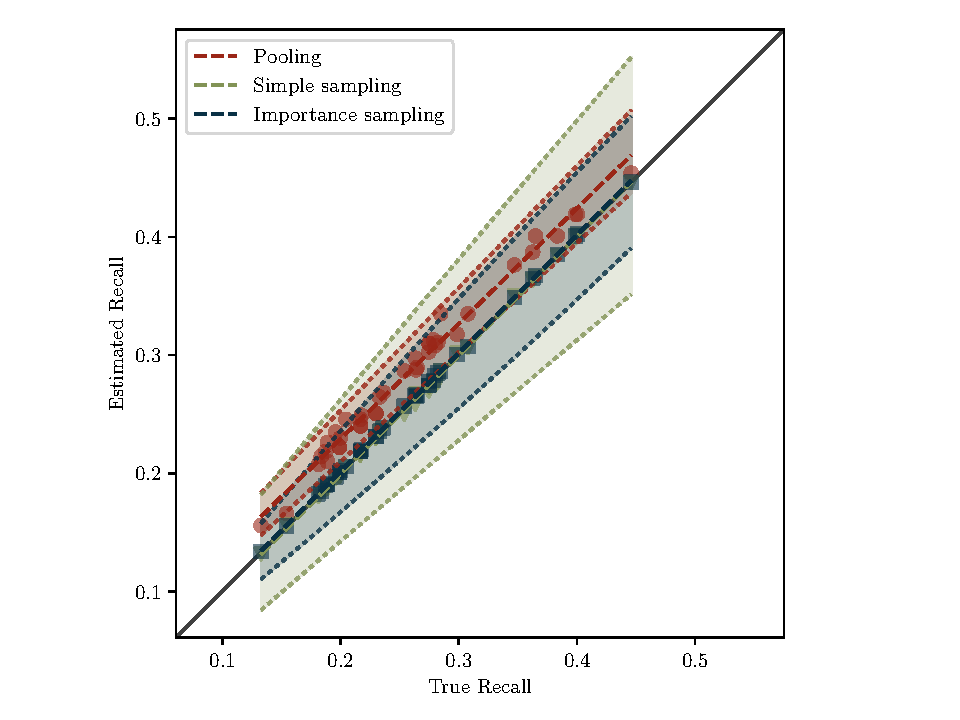
\includegraphics[width=\textwidth]{figures/simulation/simulation-r}
  \end{subfigure}
  \caption{\label{fig:simulation}
  A comparison of the pooling methodology and the simple and joint estimators on the TAC KBP 2015 challenge.
  Each point in the figure represents the mean value of estimates from 500 repeated trials, and the dotted lines show the 90\% quartile.
  Dashed trend lines indicate the mean bias of the estimation method: an unbiased system should lie on the $y = x$ line.
  Both the simple and joint estimators are unbiased, and the joint estimator is able to significantly reduce variance.
  }
\end{figure*}

\subsection{Evaluating bias and variance of the on-demand evaluation.}
Once again, we use all the system predictions from the TAC KBP 2015 evaluation and treat the labeled instances as an exhaustively annotated dataset.
To evaluate the pooling methodology, we contruct an evaluation dataset using
instances found by human annotators and labeled instances pooled from 9
randomly chosen teams (i.e.\ half the total number of participating teams), and
use this dataset to evaluate the remaining 9 teams.
On average, the pooled evaluation dataset contains between 5,000 and 6,000 labeled instances and evaluates 34 different systems (recall that each team may have submitted multiple systems).
Next, we evaluated a set of 9 randomly chosen teams with our proposed simple and joint estimators using a total of 5,000 samples.
About 150 of these samples are drawn from $\sY$, i.e.\ the complete TAC KBP 2015 evaluation data, and roughly another 150 samples from each of the systems being evaluated.
The samples are used by the simple and joint estimators to estimate precision and recall.

We repeat the above experiment 500 times and compare the estimated precision and recall with their true values in \reffig{simulation}.
The simulations once again highlight that the pooled methodology is biased, while the simple and joint estimators are not.
Furthermore, the joint estimators significantly reduce variance when compared with the simple estimators,
approximately reducing the size the 90\% confidence intervals by a factor of 2 for precision and a factor of 3 for recall.

\subsection{A mock evaluation for TAC KBP 2016}
We have implemented the on-demand evaluation framework described here as an evaluation service which research can submit their own system predictions to.
As a pilot of the service, we evaluated three distinct relation extraction systems (a pattern-based system, a supervised system and a neural network classifier) on 15,000 Newswire documents from 2016 TAC KBP evaluation.
Each system uses Stanford CoreNLP~\citep{manning2014stanford} to identify entities and the Illinois Wikifier~\citep{ratinov2011local} to perform entity linking. 
These systems were also key components of three different submissions to the official TAC KBP 2016 evaluation.

\begin{figure}[t]
  \centering
  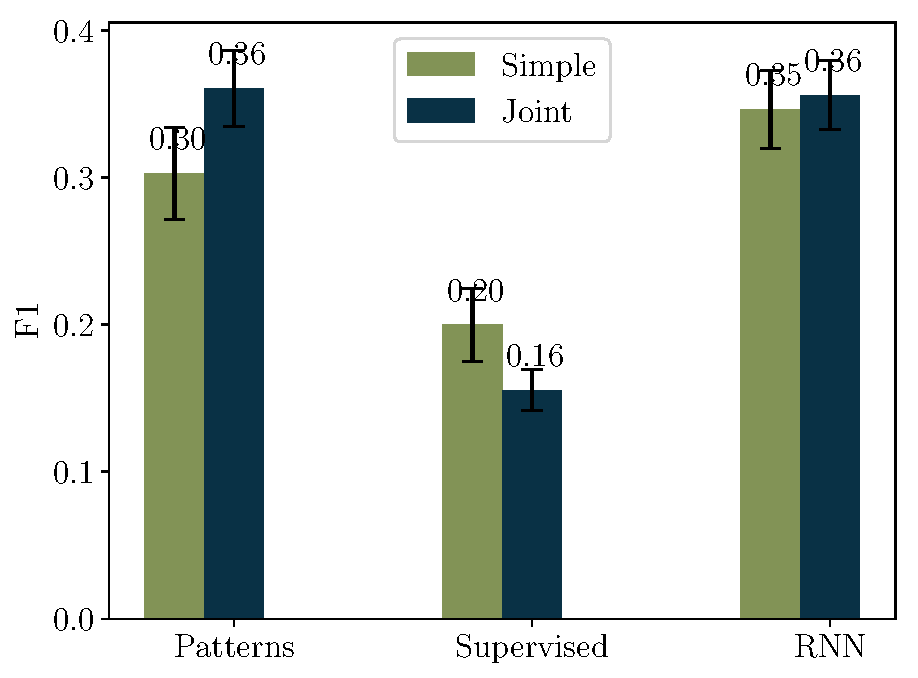
\includegraphics[width=\columnwidth]{figures/kbp2016/kbp2016_f1}
  \caption{\label{fig:evaluation-results} Results from a mock evaluation.}
\end{figure}
In total, 100 documents were exhaustively annotated for about \$2,000, and 1,000 instances from each system were labeled for about \$300 each, with 500 sampled to estimate macro-averaged relation scores and 500 were sampled to estimate macro-averaged entity scores. We manually labelled 200 relation instances from exhaustively annotated documents and observed a precision of about 75\%, which although is slightly less than 80\% obtained by annotators at LDC \cite{ellis2015overview}, was qualitatively due to improper entity spans and can be easily improved with appropriate changes to the interface. 
\reffig{evaluation-results} compares the scores obtained through on-demand evaluation of these systems with \fake{the official TAC KBP evaluation scores}.
We note that when the systems were submitted to the official TAC KBP evaluation, they included some filtering and post-processing as necessary under the evaluation guidelines, making it hard to directly compare the evaluation scores.
\ac{We need to address the discrepancy in scores here.}

